\chapter{Automatyzacja pomiarów i testów}

\section{Wymagania sprzętowe}

\noindent Sprzęt konieczny do przeprowadzenia badań:

\begin{itemize}
    \item dowolna płytka deweloperska z układem FPGA,
    \item konwerter UART/USB,
    \item komputer PC z systemem operacyjnym Linux.
\end{itemize}

\begin{figure}[H]
    \centering
    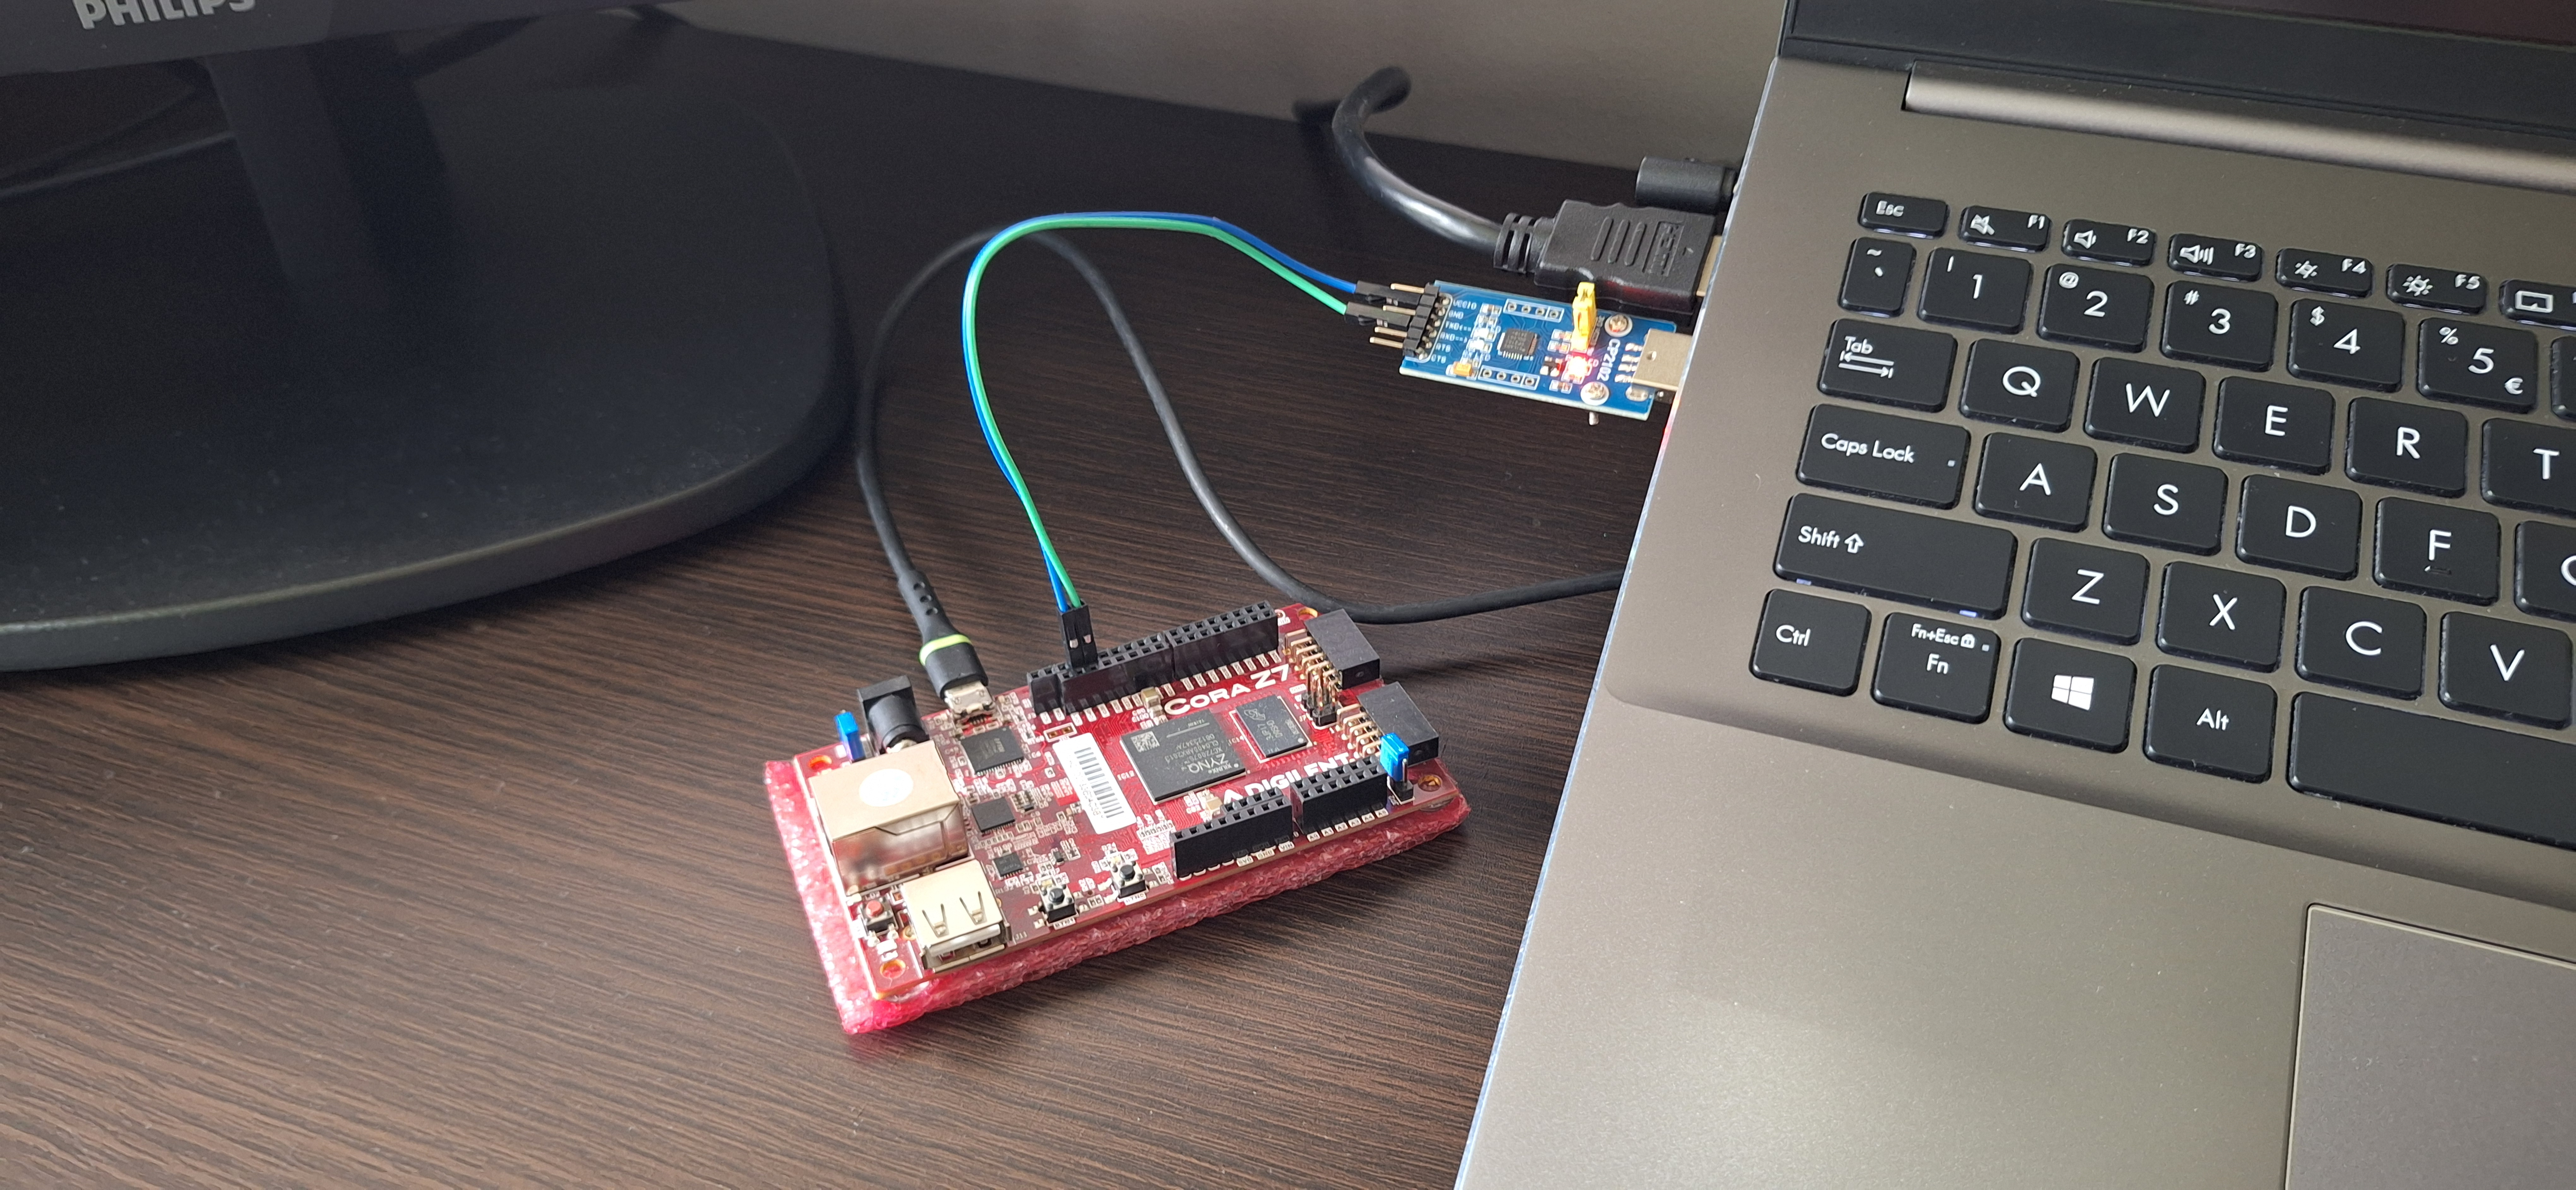
\includegraphics[width=\textwidth]{figures/AB/stacja.jpg}
    \caption{Aparatura pomiarowa}
    \label{fig:B_aparatura}
\end{figure}

\section{Zbieranie danych}

\noindent Użyteczne komendy:

\begin{description}
    \item[\texttt{sudo stty -F /dev/ttyUSB0 921600 raw -echo}] \hfill \\ 
    Konfiguracja prędkości (baudrate) portu szeregowego.
    \item[\texttt{sudo dd if=/dev/ttyUSB0 of=<file>.bin bs=1M count=100 status=progress iflag=fullblock}] \hfill Zebranie 100 MiB danych losowych do pliku binarnego.
    \item[\texttt{sudo xxd /dev/ttyUSB0}] \hfill \\ Podgląd danych na żywo.
    \item[\texttt{sudo cat /dev/ttyUSB0 | pv -r > /dev/null}] \hfill \\ Licznik prędkości (baudrate) na żywo ([x]B/s). 
\end{description}


\section{Uruchamianie pojedynczych testów}

\begin{description}
    \item[\texttt{<ENT dir>\$ ./ent <file>.bin}] \hfill \\ 
    Uruchomienie ENT.

    \item[\texttt{<NIST SP 800-22 dir>\$ ./assess 1000000}] \hfill \\ 
    Uruchomienie NIST SP 800-22.

    \item[\texttt{<NIST SP 800-90B dir>\$ ./ea\_non\_iid <file>.bin 8}] \hfill \\ 
    Uruchomienie NIST SP 800-90B.
\end{description}

\begin{figure}[H]
    \centering
    \begin{minted}[linenos, breaklines, breakanywhere]{bash}
$ ./assess 1000000
           G E N E R A T O R    S E L E C T I O N 
           ______________________________________

    [0] Input File                 [1] Linear Congruential
    [2] Quadratic Congruential I   [3] Quadratic Congruential II
    [4] Cubic Congruential         [5] XOR
    [6] Modular Exponentiation     [7] Blum-Blum-Shub
    [8] Micali-Schnorr             [9] G Using SHA-1

   Enter Choice: 0


        User Prescribed Input File: <file>.bin

                S T A T I S T I C A L   T E S T S
                _________________________________

    [01] Frequency                       [02] Block Frequency
    [03] Cumulative Sums                 [04] Runs
    [05] Longest Run of Ones             [06] Rank
    [07] Discrete Fourier Transform      [08] Nonperiodic Template Matchings
    [09] Overlapping Template Matchings  [10] Universal Statistical
    [11] Approximate Entropy             [12] Random Excursions
    [13] Random Excursions Variant       [14] Serial
    [15] Linear Complexity

         INSTRUCTIONS
            Enter 0 if you DO NOT want to apply all of the
            statistical tests to each sequence and 1 if you DO.

   Enter Choice: 1

        P a r a m e t e r   A d j u s t m e n t s
        -----------------------------------------
    [1] Block Frequency Test - block length(M):         128
    [2] NonOverlapping Template Test - block length(m): 9
    [3] Overlapping Template Test - block length(m):    9
    [4] Approximate Entropy Test - block length(m):     10
    [5] Serial Test - block length(m):                  16
    [6] Linear Complexity Test - block length(M):       500

   Select Test (0 to continue): 0

   How many bitstreams? 100

   Input File Format:
    [0] ASCII - A sequence of ASCII 0's and 1's
    [1] Binary - Each byte in data file contains 8 bits of data

   Select input mode:  1

     Statistical Testing In Progress.........
    \end{minted}
    \caption{Dialog NIST SP 800-22.}
    \label{fig:B_dialog_nist_22}
\end{figure}

\section{Struktura zbioru danych}

\begin{figure}[H]
    \centering
    % Adjust the width if your paths are very long
    \begin{minipage}{0.6\textwidth} 
        \dirtree{%
        .1 \textbf{data/1\_testy\_bazowe/2RO\_8I}/\$ tree.
        .2 false\_false.bin.
        .2 false\_true.bin.
        .2 true\_false.bin.
        .2 true\_true.bin.
        .2 \textbf{tests\_results}.
        .3 \textbf{ent}.
        .4 false\_false.log.
        .4 false\_true.log.
        .4 true\_false.log.
        .4 true\_true.log.
        .3 \textbf{nist22}.
        .4 false\_false.txt.
        .4 false\_true.txt.
        .4 true\_false.txt.
        .4 true\_true.txt.
        .4 table.txt.
        .3 \textbf{nist90}.
        .4 false\_false.log.
        .4 false\_true.log.
        .4 true\_false.log.
        .4 true\_true.log.
        .2 \textbf{utilization}.
        .3 false\_false.rpt.
        .3 false\_true.rpt.
        .3 true\_false.rpt.
        .3 true\_true.rpt.
        }
    \end{minipage}
    \caption{Struktura katalogów dla konfiguracji 2RO\_8I.}
    \label{fig:B_dir_tree}
\end{figure}

Dla każdej z badanych konfiguracji RO powstał wynikowy katalog zgodny ze schematem 
(Fig.~\ref{fig:B_dir_tree}):

\begin{itemize}
    \item \texttt{root} -- przechowuje pliki binarne z zebranymi danymi,
    \item \texttt{tests\_results} -- katalog na wyniki wszystkich testów,
    \item \texttt{ent} -- wyniki testów ENT,
    \item \texttt{nist22} -- wyniki testów NIST SP 800-22 oraz wygenerowana tabela,
    \item \texttt{nist90} -- wyniki testów NIST SP 800-90B,
    \item \texttt{utilization} -- raporty wykorzystania zasobów.
\end{itemize}

Łącznie w ramach badań zebrano:

\begin{itemize}
    \item 40 plików .bin (łącznie około 4 GB danych),
    \item 129 plików z wynikami testów .log i .txt,
    \item 40 raportów wykorzystania zasobów.
\end{itemize}

\section{Automatyzacja testów}

Wykonanie testów zostało zautomatyzowane za pomocą skryptów w języku Python:

\begin{itemize}
    \item \texttt{ent\_automation.py} -- przyjmuje ścieżkę do katalogu \texttt{root} z 
    badaną konfiguracją, wyszukuje pliki .bin, uruchamia testy i zapisuje wyniki w \texttt{root/tests\_results/ent/},
    \item \texttt{nist22\_automation.py} -- przyjmuje ścieżkę do katalogu \texttt{root} z 
    badaną konfiguracją, wyszukuje pliki .bin, uruchamia testy i zapisuje wyniki w \texttt{root/tests\_results/nist22/}, 
    \item \texttt{nist90\_automation.py} -- przyjmuje ścieżkę do katalogu \texttt{root} z 
    badaną konfiguracją, wyszukuje pliki .bin, uruchamia testy i zapisuje wyniki w \texttt{root/tests\_results/nist90/},
    \item \texttt{resource\_automation.py} -- przyjmuje ścieżkę do katalogu \texttt{data} ze 
    wszystkimi folderami różnych konfiguracji, wyszukuje pliki .rpt i zestawia 
    wyniki w jedną tabelę \LaTeX,
    \item \texttt{table\_automation.py} -- przyjmuje ścieżkę do katalogu \texttt{nist22} z 
    badaną konfiguracją, wyszukuje wyniki testów NIST SP 800-22 i zestawia je w formę 
    tabeli \LaTeX.
\end{itemize}

\begin{figure}[H]
    \centering
    \begin{minted}[linenos, breaklines, breakanywhere]{bash}
<path>/data$ python3 ent_automation.py ./1_testy_bazowe/2RO_8I/
ENT processing false_false.bin...
Entropy = 5.322542 bits per byte.
Saved -> <path>/data/1_testy_bazowe/2RO_8I/tests_results/ent/false_false.log
ENT processing false_true.bin...
Entropy = 7.999742 bits per byte.
Saved -> <path>/data/1_testy_bazowe/2RO_8I/tests_results/ent/false_true.log
ENT processing true_false.bin...
Entropy = 7.168778 bits per byte.
Saved -> <path>/data/1_testy_bazowe/2RO_8I/tests_results/ent/true_false.log
ENT processing true_true.bin...
Entropy = 7.999997 bits per byte.
Saved -> <path>/data/1_testy_bazowe/2RO_8I/tests_results/ent/true_true.log
    \end{minted}
    \caption{Uruchomienie skryptu automatyzacji testów ENT dla /1\_testy\_bazowe/2RO\_8I.}
    \label{fig:B_automatyzacja_ent_python}
\end{figure}